\subsection{Vocabulario}

A continuación se define una parte del vocabulario común que se utiliza al estudiar grafos.

\subsubsection{Orden y tamaño}

El \concept{orden} de un grafo \(G\), denotado por \(|G|\), se define como el número de vértices: \[|G| = |V|.\] Es usual usar \(n\) para \(n = |G|\).

Se define el \concept{tamaño} de \(G\), denotado por \(\varepsilon(G)\) o simplemente por \(\varepsilon\), como el número de arcos: \[\varepsilon = |E|.\]

\subsubsection{Incidencia, adyacencia y vecindario}
\label{sec:adyacencia}

Se dice que un arco \(\{u,v\}\) (o simplemente \(uv\)) \concept{une} (\textit{joins}) los vértices \(u\) y \(v\). Se dice que \(u\) y \(v\) son \concept{incidentes} a el arco \(uv\), al igual que el arco \(uv\) es \concept{incidente} tanto a \(u\) como a \(v\).

Más aún, se dice los vértices \(u\) y \(v\) son \concept{adyacentes} o \concept{vecinos}. Se denota que \(u\) y \(v\) son adyacentes por \[u \longrightarrow v.\]
En un grafo \emph{no dirigido}, es lo mismo escribir que \(u\longrightarrow v\), que \(v \longrightarrow u\) y que \(\{u,v\} \in E\).

El conjunto de los vértices adyacentes a \(v\) se denomina el \concept{vecindario} de \(v\) y se denota por \(\Gamma(v)\). \[\Gamma(v) = \{x \ | \ v \longrightarrow x\}\] Se dice que \(\Gamma(v)\) es el \concept{vecindario abierto} de \(v\) y que \(\Gamma(v) \cup \{v\}\) es el \concept{vecindario cerrado}.

Sea \(S \subseteq V\) un conjunto de vértices de \(G\), la notación \(v\longrightarrow S\) indica que \(v\) es adyacente a cada vértice de \(S\), \(v\longrightarrow x\) para todo \(x \in S\). Naturalmente, si \(v \longrightarrow S\), entonces \(S \subseteq \Gamma(v)\).

Si dos arcos comparten un vértice, también se dice de los arcos que son \concept{adyacentes}.

\subsubsection{Predecesor y sucesor}
\label{sec:predecesor_sucesor}

Para grafos \emph{dirigidos}, el concepto de adyacencia no basta para indicar la dirección de los arcos.

Se dice que \(u\) es \concept{predecesor} de \(v\) si hay un arco de \(u\) a \(v\), \((u, v) \in E\). En ese caso, se dice también que \(v\) es \concept{sucesor} de \(u\). Ambas cosas se denotan por \(uv\) o por \[u \longrightarrow v.\]Análogo a antes, la notación \(u\longrightarrow S\) indica que \(u\) es predecesor de cada vértice en \(S\subseteq V\), \(u\longrightarrow x\) para todo \(x \in S\).

\subsubsection{Grado}
\label{sec:grado}

El \concept{grado} (\textit{degree}) de un vértice se define como el número de vértices adyacentes a él. Equivalentemente, es el número de vértices en su vecindario (abierto).

El grado de \(v\) se denota por \(d(v)\): \[d(v) = |\Gamma(v)|.\] El grado de un vértice puede ser 0, si no tiene vértices adyacentes. En ese caso, se dice que el vértice está \concept{aislado} (\textit{isolated}).

Se denota el mínimo grado de todos los vértices de \(G\) por \(\delta(G)\) (o solo \(\delta\)). Similarmente, el máximo grado se denota por \(\Delta(G)\) o \(\Delta\).

Si para algún grafo sucede que \(\delta = \Delta = k\), entonces todos los vértices tienen igual grado, \(k\). En ese caso, se dice que el grafo es \concept{regular} de grado \(k\).

Por ejemplo, todo grafo regular de grado \(3\) se puede dibujar con forma de cubo. Más formalmente, como se verá posteriormente, se puede decir que todo grafo regular de grado \(3\) es isomorfo al grafo cubo.

\begin{center}
  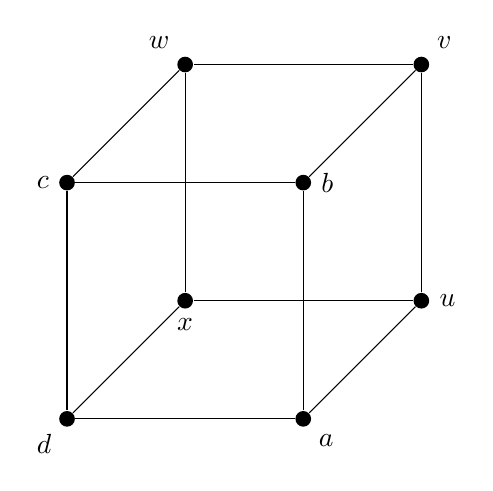
\begin{tikzpicture}[scale=1,
    vertex/.style={circle, fill=black, inner sep=2pt}]
    % Bottom face (front square): a (down-right), b (up-right), c (up-left), d (down-left)
    \node[vertex, label=below left:\(d\)]   (d) at (0,   0)   {};
    \node[vertex, label=below right:\(a\)]  (a) at (3,   0)   {};
    \node[vertex, label=right:\(b\)]        (b) at (3,   3)   {};
    \node[vertex, label=left:\(c\)]         (c) at (0,   3)   {};
    \draw (a) -- (b) -- (c) -- (d) -- (a);

    % Top face (back square, offset up-right): 
    \node[vertex, label=below:\(x\)]        (x) at (1.5, 1.5) {};
    \node[vertex, label=right:\(u\)]        (u) at (4.5, 1.5) {};
    \node[vertex, label=above right:\(v\)]  (v) at (4.5, 4.5) {};
    \node[vertex, label=above left:\(w\)]   (w) at (1.5, 4.5) {};
    \draw (u) -- (v) -- (w) -- (x) -- (u);
    
    % Edges mapping faces
    \draw (a) -- (u);
    \draw (b) -- (v);
    \draw (c) -- (w);
    \draw (d) -- (x);
  \end{tikzpicture}
\end{center}
